%\documentclass{beamer}
\documentclass[aspectratio=169]{beamer}

% SETUP =====================================
\usepackage[T1,T2A]{fontenc}
\usepackage[utf8]{inputenc}
\usepackage[russian]{babel}
\usepackage{hyperref}
\usepackage{listings}
\usepackage{marvosym}
\usepackage{minted} 
\usepackage{../../beamerthemeslidesgeneric}
% SETUP =====================================

\title{Scala Introduction}
\author{Mikhail Mutcianko, Alexey Shcherbakov}
\institute{СПБгУ, СП}
\date{\today}

\begin{document}

\frame{\titlepage}

\section{Intro}

\begin{frame}{Disclaimer}
  \begin{block}{Prior knowledge}
    You are expected to alrady posess certain knowledge from previous programming courses.
    We will not explain basic programming concepts like classes, functions, variables etc\ldots
  \end{block}
  \pause
  \begin{itemize}
    \item knowledge of OOP and FP
      \pause
    \item knowledge of JVM platform
      \pause
    \item knowledge of algorithms and data structures from CS
  \end{itemize}
\end{frame}

\begin{frame}{What is Scala?}
  Scala is a general-purpose programming language providing support for
  functional programming and a strong static type system. Designed to be concise, many of Scala's
  design decisions aimed to address criticisms of Java.
\end{frame}

\section{History}

\begin{frame}{Java Generics}
  \begin{itemize}
    \item Java had no generics pre 1.4
    \item May 1999: Sun proposes to Add Generics to Java, based on GJ
    \item May 2001: Sun releases prototype for Adding Generics to Java
    \item January 2003: Generics headed for inclusion in Java 1.5
  \end{itemize}
\end{frame}

\begin{frame}[fragile]{GJ}{A Generic Java Language Extension}
  \begin{block}{WTF GJ?}
    GJ is an extension of the Java programming language that supports generic types
  \end{block}
  \only<1>{
    \begin{itemize}
      \item support for generics
      \item superset of the Java programming language
      \item compatible with existing libraries
      \item efficient translation by erasure
    \end{itemize}
  }
  \only<2>{
    \vfill
    \begin{center}
      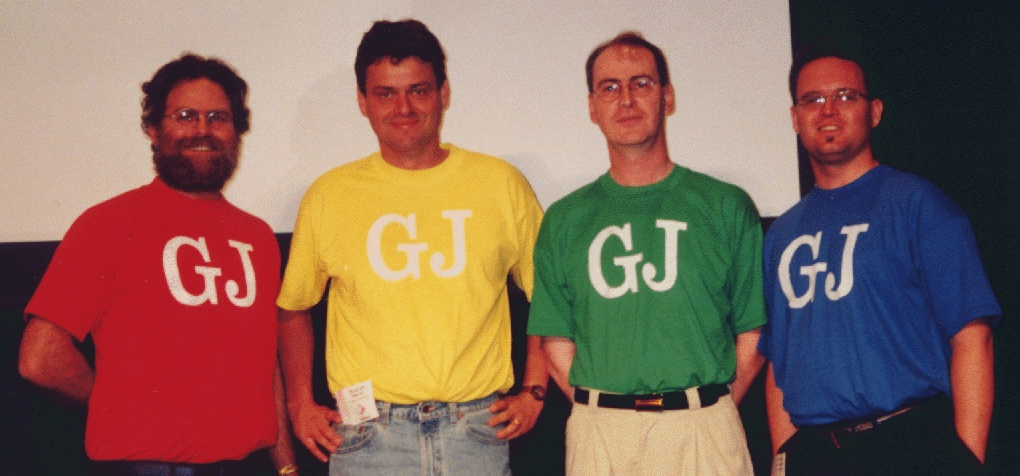
\includegraphics[scale=0.2]{gj-front-full.jpg}
    \end{center}
  }
\end{frame}

\begin{frame}{Pizza}
  \begin{itemize}
    \item move some ideas from FP into the Java space
    \item take three features from functional programming:
      \begin{itemize}
        \item generics
        \item higher-order functions
        \item pattern matching
      \end{itemize}
    \item work on Pizza has more or less stopped since 2002 \large\Cross
  \end{itemize}
\end{frame}

\begin{frame}[fragile]{Pizza}
  \begin{lstlisting}[style=scala,language=java]
public final class Main {
  public int main(String args[]) {
    System.out.println(
      new Lines(new DataInputStream(System.in))
        .takeWhile(nonEmpty)
        .map(fun(String s) -> int { return Integer.parseInt(s); })
        .reduceLeft(0, fun(int x, int y) -> int { return x + y; }));
        while(x == 0) { map.create.newInstance() }
  }
}
  \end{lstlisting}
\end{frame}

\begin{frame}{Scala}{origins}
  \begin{exampleblock}{}
    {\large ``I wanted to design a language that was different from Java,
              it would always connect to the Java infrastructure — to the JVM and its libraries.''}
    \vskip3mm
    \hspace*\fill{\small--- Martin Odersky}
  \end{exampleblock}
\end{frame}

\begin{frame}{Scala}{origins}
\begin{itemize}
  \item \texttt{Funnel} --- first attempt, beautiful but too abstract \large\Cross
  \item midway between academic Funnel, and pragmatic but restrictive GJ
  \item first public release of \texttt{Scala} in 2003
  \item large redesign in early 2006
\end{itemize}
\end{frame}

\begin{frame}{Scala}{EPFL}
  \begin{columns}
    \column{0.5\textwidth}
    \centering\scalebox{-1}[1]{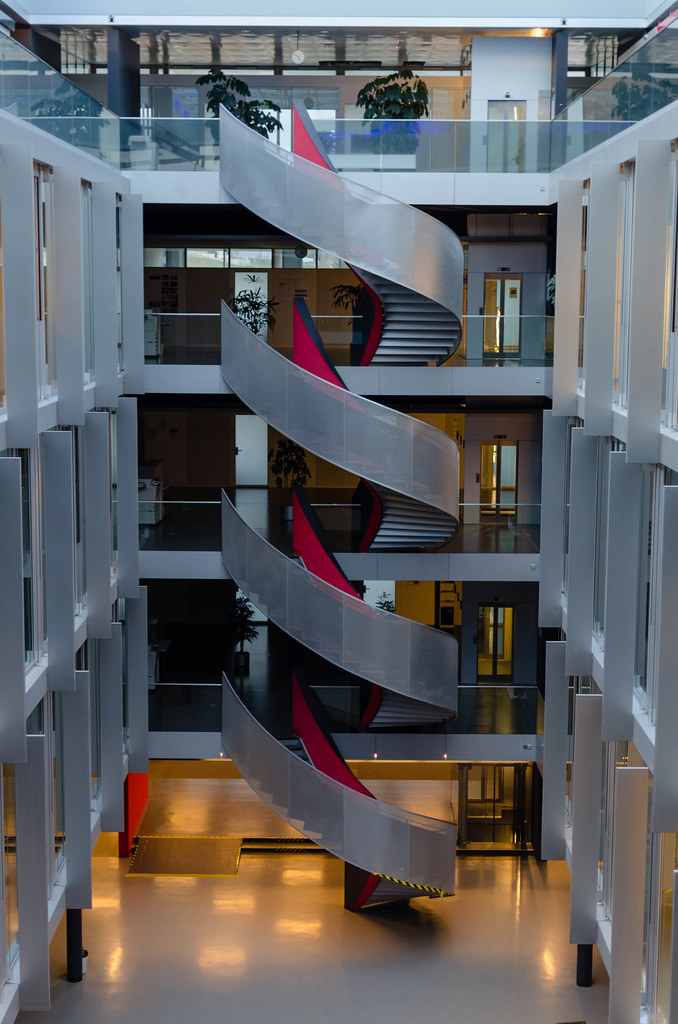
\includegraphics[height=0.9\textheight]{stair.jpg}}
    \column{0.5\textwidth}
    \centering
\includegraphics[height=0.7\textheight]{scala-logo.pdf}
  \end{columns}
\end{frame}

\begin{frame}{Academic vs Industrial}
  \begin{columns}
    \column{0.5\textwidth}
    \begin{block}{Academic}
      \begin{itemize}
        \item Haskell
        \item Agda
        \item Idris
        \item \ldots
      \end{itemize}
    \end{block}
    \column{0.5\textwidth}
    \begin{block}{Industrial}
      \begin{itemize}
        \item Java
        \item Python
        \item \alert{Scala} ?
        \item \ldots
      \end{itemize}
    \end{block}
  \end{columns}
\end{frame}

\section{Scala benefits}

\begin{frame}{Multiparadigm}
  \vspace*{-8pt}
  \begin{columns}[T]
    \pause
    \column{0.5\textwidth}
    \begin{block}{OOP \& Imperative}
      \vspace*{-10pt}
      \begin{itemize}
        \item traits \& objects
        \item trait mixins
        \item abstract overrides
        \item self types
        \item \ldots
      \end{itemize}
    \end{block}
    \pause
    \column{0.5\textwidth}
    \begin{block}{Functional}
      \vspace*{-10pt}
      \begin{itemize}
        \item type inference
        \item lambdas
        \item higher-order functions
        \item lazy evaluation
        \item immutability
        \item pattern matching
        \item currying
        \item ADTs
        %\item \ldots
      \end{itemize}
    \end{block}
  \end{columns}
\end{frame}

\begin{frame}{Type Safety}
  \begin{block}{What is type safety?}
    Type-safety is making use of what we know of our values at compile-time to minimize the
    consequences of most mistakes.
  \end{block}
  \pause
  \begin{itemize}
    \item monads
    \item ADTs
    \item immutability
    \item value types
    \item \ldots
  \end{itemize}
\end{frame}

\begin{frame}{Libraries and Frameworks}
  \begin{itemize}
    \item Akka --- actor model implementation
      \pause
    \item Spark --- cluster computing system
      \pause
    \item Shapeless --- type class \& dependent types
      \pause
    \item Cats, Scalaz --- principled FP
      \pause
    \item Play! --- full-scale web
      \pause
    \item \ldots
  \end{itemize}
\end{frame}

\begin{frame}{Real world}{Banks}
  \begin{block}{Why Scala?}
    Banking and Financial Institute majorly concerns for security, stability and sustainability
    support in the long terms. Scala will satisfy this needs.
  \end{block}
  \begin{itemize}
    \item Tinkoff
    \item JP Morgan
    \item Credit Suisse
    \item Morgan Stanley
    \item \ldots
  \end{itemize}
\end{frame}

\section{Scala responsibility}

\begin{frame}{Compilation times}
  \begin{itemize}
    \item using macros
    \item overuse of implicits
    \item overuse of libraries with macros and implicits
  \end{itemize}
\end{frame}

\begin{frame}[fragile]{Codestyle}{Infix notation}
\begin{lstlisting}[style=scala,language=scala]
def main(args:Array[String]) = {
  10 PRINT "Enter a number"
  20 INPUT n
  30 PRINT "Square root of " % "n is " % SQRT(n)
  40 END
  RUN
}
\end{lstlisting}
\end{frame}

% https://gist.github.com/razie/595556
\begin{frame}[fragile]{Codestyle}{Types}
\begin{lstlisting}[style=scala,language=scala]
trait WRGraph[N <: GNode[N, L], L <: GLink[N]] extends GNode[N, L] { this: N =>

def combo[AA <: A >: B <% String <% Int : M : Ordering] = ???
...
}
\end{lstlisting}
\end{frame}

\begin{frame}{Codestyle}
  \begin{itemize}
    \item implicit hell
    \item mixing codestyles
    \item \ldots
  \end{itemize}
\end{frame}

\section{Hands-on}

\begin{frame}{IDEA}
\centering\Large Install Scala plugin
\end{frame}

\begin{frame}[fragile]{SBT}
\begin{verbatim}
$ sbt
sbt:project> ;compile;test:compile
...
sbt:project> run
sbt:project> test
sbt:project> console
\end{verbatim}
\end{frame}

\section{Practice}

\end{document}

